\documentclass[12pt]{book}
\usepackage[utf8]{inputenc}
\usepackage[english]{babel}	% hyphenation and content headings  %%LOCALIZE

\usepackage[T1]{fontenc}		% Allow Swedish, German etc. letters
\DeclareTextCommand{\nobreakspace}{T1}{\leavevmode\nobreak\ }


\usepackage{titling}
\usepackage[left=2cm, right=2cm,bottom=3cm,top=2cm, paperwidth=297mm, paperheight=210mm, twoside=false]{geometry}

\usepackage[scaled]{helvet}
%\usepackage{tgheros} %alternative to helvet
\renewcommand{\familydefault}{\sfdefault}
\usepackage{sectsty}
\allsectionsfont{\sffamily}
\usepackage[scaled=1.02]{inconsolata}
%\usepackage[scaled]{beramono} %alternative to inconsolata

\usepackage{url}
\usepackage[hidelinks]{hyperref}
\usepackage{wrapfig}
\usepackage{titlepic, graphicx}
\usepackage[usenames,dvipsnames]{xcolor}
\usepackage{array} %to center table cells
\usepackage{parskip} %to have noindent and space between paras
\usepackage{tikz}

\usepackage{titlesec}
\titleformat{\chapter}[hang]{\bf\fontsize{40}{40}\selectfont\centering\vskip-13mm}{}{0pt}{\bf\fontsize{40}{40}\selectfont}
\titleformat{\section}[hang]{\bf\fontsize{24}{24}\selectfont}{}{0pt}{\bf\fontsize{24}{24}\selectfont}
\titlespacing\chapter{0pt}{20pt plus 10pt minus 10pt}{20pt plus 10pt minus 10pt}
\titlespacing\section{0pt}{10pt plus 4pt minus 2pt}{0pt plus 4pt minus 2pt}

\usepackage{multicol}

\usepackage{listings}
\lstset{literate=%
%swedish and german letters
{Å}{{\AA}}1
{Ä}{{\"A}}1
{Ö}{{\"O}}1
{Ü}{{\"U}}1
{ß}{{\ss}}1
{ü}{{\"u}}1
{å}{{\aa}}1
{ä}{{\"a}}1
{ö}{{\"o}}1
%danish letters
{æ}{{\ae}}1
{ø}{{\o}}1
{Æ}{{\AE}}1
{Ø}{{\O}}1
}            
% "define" Scala
\lstdefinelanguage{scala}{
  morekeywords={abstract,case,catch,class,def,%
    do,else,extends,false,final,finally,%
    for,forSome,if,implicit,import,lazy,match,%
    new,null,object,override,package,%
    private,protected,return,sealed,%
    super,this,throw,trait,true,try,%
    type,val,var,while,with,yield},
  otherkeywords={=>,<-,<\%,<:,>:,@},
  sensitive=true,
  morecomment=[l]{//},
  morecomment=[n]{/*}{*/},
  morestring=[b]",
  morestring=[b]',
  morestring=[b]"""
}
\usepackage{color}
\definecolor{dkgreen}{rgb}{0,0.6,0}
\definecolor{gray}{rgb}{0.5,0.5,0.5}
\definecolor{dkgray}{rgb}{0.3,0.3,0.3}
\definecolor{mauve}{rgb}{0.58,0,0.82}
 
% Default settings for code listings
\lstset{frame=none, 
  language=scala,
  aboveskip=3mm,
  belowskip=3mm,
  %framesep=2cm,xleftmargin=-10pt,xrightmargin=10pt,
  showstringspaces=false,
  columns=flexible,%flexible ,%fixed
  basicstyle={\ttfamily\selectfont},
  keywordstyle=\bf\ttfamily\selectfont\color{blue},
  commentstyle=\color{dkgreen},
  stringstyle=\color{mauve},
  breaklines=false,
  breakatwhitespace=false,
  tabsize=2,
  numbers=none,stepnumber=1, numbersep=8pt, numberstyle=\small\color{gray}
}

\title{\fontsize{40}{40}\bf\sffamily\selectfont Challenges with Kojo} %%%LOCALIZE
\author{Editor: Björn Regnell \\ \bf www.lth.se/code} %%%LOCALIZE
\titlepic{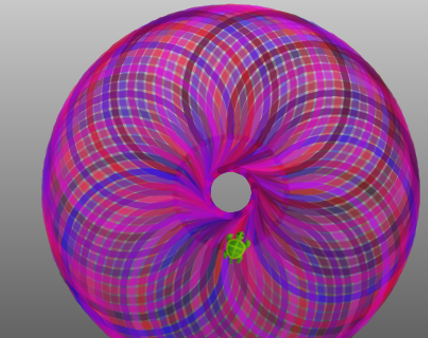
\includegraphics[height=8cm]{../img/cover}}
\date{}
\renewcommand{\thechapter}{} % removes chapter numbers also in table of contents

\begin{document}
\maketitle
\newpage
\thispagestyle{empty}

{ \vspace{250mm}\fontsize{11}{11}\flushleft\selectfont 
\vspace*{\fill}

\begin{center}
\Huge {\bf Challenges with Kojo}\\
\Large {\bf Version}: \today{ }
\end{center}
\vskip7cm

\large

\includegraphics{../img/cc.png}

License: Creative Commons {\it Attribution-NonCommercial-ShareAlike 4.0 International} 
\href{http://creativecommons.org/licenses/by-nc-sa/4.0/}{CC BY-NC-SA 4.0}

Editor: Björn Regnell\\
Contributors: Björn Regnell, Lalit Pant, Sandra Nilsson, Maja Johansson, ... \\
\textcopyright{ }Björn Regnell, Lund University, 2015 \\
\url{http://lth.se/programmera}
}  %%%LOCALIZE

\newpage
\begin{multicols}{3}
\addtocontents{toc}{\protect\thispagestyle{empty}}
\tableofcontents 
\mainmatter
\end{multicols}

\fontsize{16}{18}\selectfont\raggedright

\chapter{About Kojo}
\begin{multicols}{2}
\section*{\color{black}What is Kojo?}
Kojo is an app that can help you learn how to program. With Kojo you can code using the modern and powerful programming language {\bf\color{blue}Scala}. Kojo is free and available for Linux, Windows and Mac.
\section*{\color{black}Where can I find Kojo?}
Download Kojo here: 
\\

\href{http://www.kogics.net/kojo-download}{www.kogics.net/kojo-download}
\\

Read more here: 
\\

\href{http://www.kogics.net/kojo}{www.kogics.net/kojo}

\columnbreak

\begin{center}
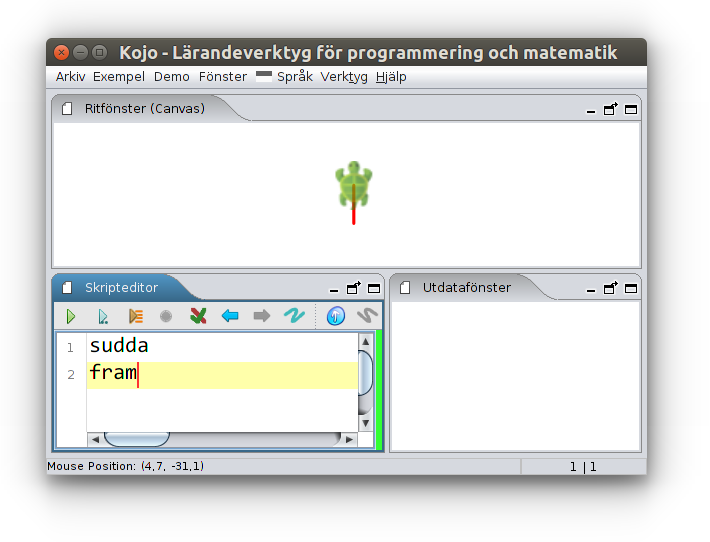
\includegraphics[width=14.0cm]{../img/kojo.png}
\end{center}

\end{multicols}

\chapter{Your first program}
\begin{multicols}{2}
\section*{\color{BrickRed}Challenge:}
Write the following in the Kojo script editor window:

\begin{lstlisting}[basicstyle={\ttfamily\fontsize{30}{36}\selectfont},numbers=none]
clear
forward
\end{lstlisting}
        
Press the green play button 

\includegraphics[width=1.0cm]{../img/play.png}
\\

to run your program.
\\

\vskip 5.0em

\columnbreak

\begin{center}
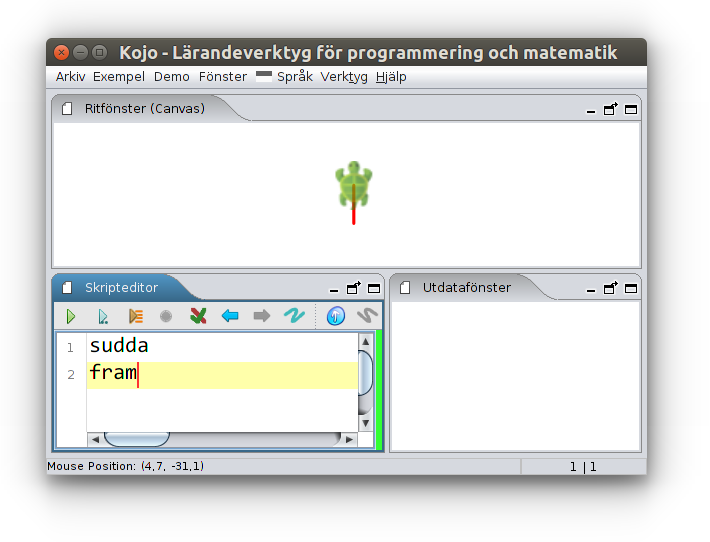
\includegraphics[width=14.0cm]{../img/fram.png}
\end{center}

\end{multicols}

\chapter{Draw a square}
\begin{multicols}{2}

\begin{lstlisting}[basicstyle={\ttfamily\fontsize{30}{36}\selectfont},numbers=none]
clear
forward
right
\end{lstlisting}
        
If you write \lstinline{left} or \lstinline{right} the turtle will change direction.
\section*{\color{BrickRed}Challenge:}
Extend the program so that it makes a square.

\columnbreak

\begin{center}
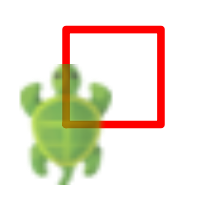
\includegraphics{../img/square.png}
\end{center}

\end{multicols}

\chapter{Draw stairs}
\begin{multicols}{2}

\begin{lstlisting}[basicstyle={\ttfamily\fontsize{30}{36}\selectfont},numbers=none]
clear
forward; left
forward; right
\end{lstlisting}
        
\vskip 1.0em
With semicolon \lstinline{;} between the commands, you could have several commands on the same line.
\section*{\color{BrickRed}Challenge:}
Extend the program so that it makes stairs.

\columnbreak

\begin{center}
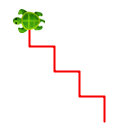
\includegraphics{../img/stairs.png}
\end{center}

\end{multicols}

\chapter{Make a loop}
\begin{multicols}{2}

\begin{lstlisting}[basicstyle={\ttfamily\fontsize{30}{36}\selectfont},numbers=none]
clear
repeat(4){ forward; right }
\end{lstlisting}
        
\section*{\color{BrickRed}Challenge:}


\begin{itemize}

\item {What will happen if you change 4 to 100?}
\item {Draw stairs with 100 steps.}

\end{itemize}



\columnbreak

\begin{center}
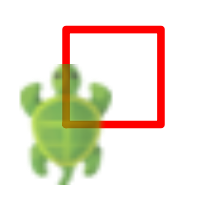
\includegraphics{../img/square.png}
\end{center}

\end{multicols}

\chapter{Draw a character}
\begin{multicols}{2}
\section*{\color{BrickRed}Challenge:}
Draw a character of your choice.
\section*{\color{OliveGreen}Tip:}

\begin{lstlisting}[basicstyle={\ttfamily\fontsize{20}{24}\selectfont},numbers=none]
hop
left(180)
forward(300)
hop(100)
jumpTo(25,-28)
write("FELIX is awesome")
setPenColor(purple)
setFillColor(green)
\end{lstlisting}
        
You can see the turtle's position down to the left while moving the mouse in the Canvas:

\includegraphics[width=6.0cm]{../img/mousepos.png}


\columnbreak


\begin{center}
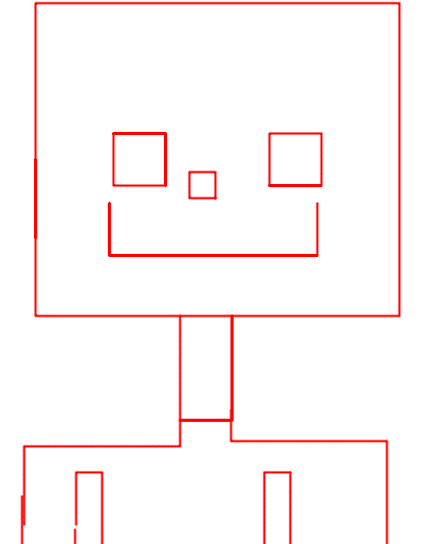
\includegraphics[width=4.5cm]{../img/man.png}
\end{center}

\vskip 2.0em
\begin{center}
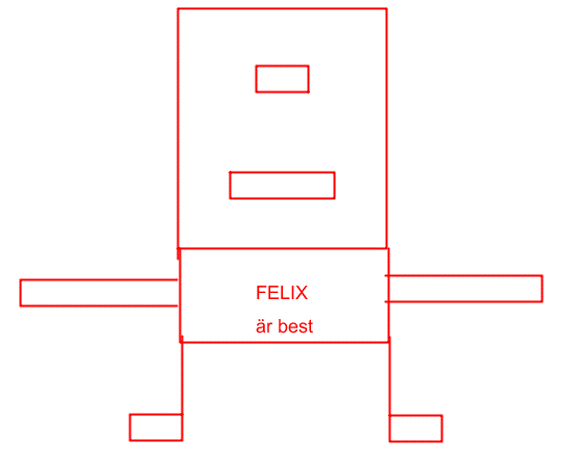
\includegraphics[width=9.0cm]{../img/alien.png}
\end{center}

\end{multicols}

\chapter{How fast is your computer?}The first electronic computer was called {\bf ENIAC} and could count up to 5000 in a second.\\
In Kojo there is a function \lstinline{räknaTill} that measures how fast the computer counts.\\
When I run \lstinline{räknaTill(5000)} on my fast computer, the following appears in the output window:

\begin{lstlisting}[numbers=none]

*** Räknar från 1 till ... 5000 *** KLAR!
Det tog 0.32 millisekunder.
      
\end{lstlisting}
        
\section*{\color{BrickRed}Challenge:}


\begin{itemize}

\item {Run \lstinline{räknaTill(5000)} and check if your computer is faster than mine.}
\item {How long does it take for your computer to count up to a million?}
\item {How much can your computer count to in a second?}

\end{itemize}


\chapter{Track the program}
\begin{multicols}{2}
\section*{\color{BrickRed}Challenge:}


\begin{itemize}

\item {Write a program that draws stairs.}
\item {Press the orange play button.}
\item {Press on one of the commands: \lstinline{CALL fram}. What happens in the Canvas?}
\item {When a part of the program is marked in blue, only that part will run when you press the play button. You can unmark the code if you click next to the code that is marked. }
\item {Add more commands to your program and observe what happens when you track it.}
\item {Close the window {\it Program tracker} when you're done.}

\end{itemize}



\columnbreak

\begin{center}
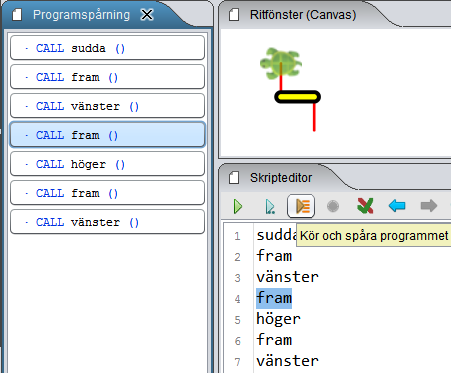
\includegraphics{../img/trace.png}
\end{center}

\end{multicols}

\chapter{Write your own function with \lstinline{def}}With \lstinline{def} you can write your own {\it functions} and choose their names.

\begin{lstlisting}[basicstyle={\ttfamily\fontsize{20}{24}\selectfont},numbers=none]
def square =  repeat(4){ forward; right }  

clear
square    //use your square-function
hop
square
\end{lstlisting}
        
\section*{\color{BrickRed}Challenge:}


\begin{itemize}

\item {Change the color of the squares.}
\item {Make several squares.}

\end{itemize}


\section*{\color{OliveGreen}Tip:}

\begin{lstlisting}[numbers=none]
setFillColor(green); setPenColor(purple)
\end{lstlisting}
        
\chapter{Stack squares}
\begin{multicols}{2}
\section*{\color{BrickRed}Challenge:}
Make a stack of 10 squares.
\section*{\color{OliveGreen}Tip:}
\vskip 1.0em

\begin{lstlisting}[numbers=none]
def square =  repeat(4){ forward; right }  

clear; setAnimationDelay(100)
repeat(10){ ??? }
\end{lstlisting}
        

\columnbreak

\begin{center}
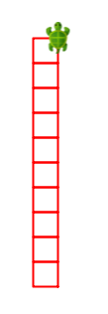
\includegraphics{../img/square-column.png}
\end{center}

\end{multicols}

\chapter{Make a stack-function}
\begin{multicols}{2}
\section*{\color{BrickRed}Challenge:}
Make a function called \lstinline{stack}, that draws a stack of 10 squares.
\section*{\color{OliveGreen}Tip:}

\begin{lstlisting}[numbers=none]
def square = repeat(4){ forward; right }  
def stack = ???

clear; setAnimationDelay(100)
stack
\end{lstlisting}
        

\columnbreak

\begin{center}
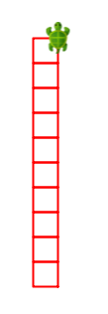
\includegraphics{../img/square-column.png}
\end{center}

\end{multicols}

\chapter{Make a grid}
\begin{multicols}{2}
\section*{\color{BrickRed}Challenge:}
Make a grid of 10*10 squares.
\section*{\color{OliveGreen}Tip:}


\begin{itemize}

\item {Use your stack-function that you created earlier.}
\item {You can jump backwards a whole column with \lstinline{hop(-10 * 25)}}
\item {You can then jump to the right position with \lstinline{right; hop; left}}

\end{itemize}



\columnbreak

\begin{center}
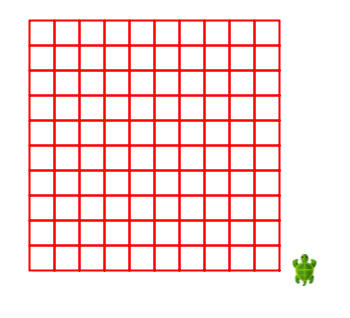
\includegraphics{../img/square-grid.png}
\end{center}

\end{multicols}

\chapter{square med parameter}
\begin{multicols}{2}
\section*{\color{BrickRed}Challenge:}
Draw squares in different sizes.
\section*{\color{OliveGreen}Tip:}
Give your function a {\it parameter},\\
called \lstinline{sideLength} of the type \lstinline{Int}:

\begin{lstlisting}[basicstyle={\ttfamily\fontsize{16}{19}\selectfont},numbers=none]
def square(sideLenght : Int) = 
  repeat(4){ forward(sideLength); right }

clear; setAnimationDelay(100); invisible
square(100) 
square(70)
square(40)
\end{lstlisting}
        
You can change the color with:\\
\lstinline{setFillColor(blue); setPenColor(pink)}


\columnbreak


\begin{center}
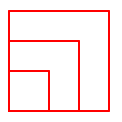
\includegraphics[width=5.0cm]{../img/square-param.png}
\end{center}

\begin{center}

\includegraphics[width=5.0cm]{../img/square-param-color.png}
\end{center}

\end{multicols}

\chapter{Draw a square character}\section*{\color{BrickRed}Challenge:}
Draw a character with squares of different sizes.
\\


\begin{tikzpicture}[overlay]
\node at (20.0cm,-1.0cm) {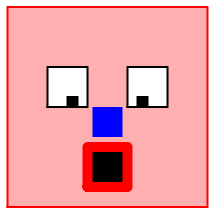
\includegraphics[width=5.5cm]{../img/square-man.png}};
\end{tikzpicture}
  
\section*{\color{OliveGreen}Tip:}

\begin{lstlisting}[basicstyle={\ttfamily\fontsize{14}{17}\selectfont},numbers=none]
def square(x: Int, y: Int, sideLength: Int) = {
  jumpTo(x, y)
  repeat(4) { forward(sideLength); right }
}
def head(x: Int, y: Int) = { setFillColor(pink); setPenColor(red); square(x, y, 200) }
def eye(x: Int, y: Int) = { setFillColor(white); setPenColor(black); square(x, y, 40) }
def pupil(x: Int, y: Int) = { setFillColor(black); setPenColor(black); square(x, y, 10) }
def nose(x: Int, y: Int) = { setFillColor(blue); setPenColor(noColor); square(x, y, 30) }
def mouth(x: Int, y: Int) = { setPenThickness (10); setFillColor(black); setPenColor(red); square(x, y, 40) }

clear; setAnimationDelay(20); invisible
head(0, 0)
eye(40, 100); pupil(60, 100)
???
\end{lstlisting}
        
\chapter{Draw a polygon}\section*{\color{BrickRed}Challenge:}


\begin{itemize}

\item {Try out the code below. Draw different kinds of polygons.}
\item {Add a parameter \lstinline{sideLength} and draw polygons of different sizes.}
\item {How large does n have to be to make it look like a circle?}

\end{itemize}


\section*{\color{OliveGreen}Tip:}

\begin{lstlisting}[basicstyle={\ttfamily\fontsize{18}{22}\selectfont},numbers=none]
def polygon(n:Int) = repeat(n){
  forward(100)
  left(360.0/n)
}

clear; setAnimationDelay(100)
polygon(7)
\end{lstlisting}
        

\begin{tikzpicture}[overlay]
\node at (20.0cm,3.5cm) {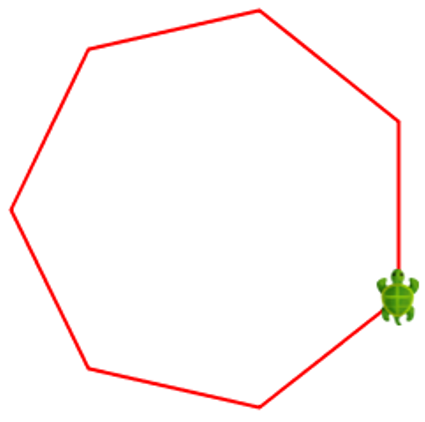
\includegraphics[width=8.0cm]{../img/polygon.png}};
\end{tikzpicture}
  
\chapter{Draw several polygons}\section*{\color{BrickRed}Challenge:}


\begin{itemize}

\item {Try out the program below.}
\item {Try to change the amount of sides and the angle.}
\item {Fill the polygons with different colors.}

\end{itemize}



\begin{tikzpicture}[overlay]
\node at (22.0cm,-0.5cm) {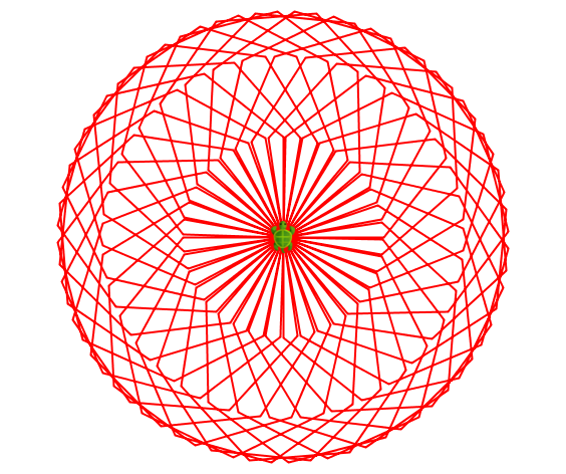
\includegraphics[width=11.0cm]{../img/polygons-circle.png}};
\end{tikzpicture}
  

\begin{lstlisting}[basicstyle={\ttfamily\fontsize{16}{19}\selectfont},numbers=none]
def polygon(n: Int, sideLength: Int) = repeat(n){
  forward(sideLength)
  left(360.0/n)
}
def rotate(n: Int, heading: Int, sideLength: Int) = 
  repeat(360/heading){ polygon(n, sideLength); left(heading) }

clear; setAnimationDelay(5)
rotate(7, 10, 100)
\end{lstlisting}
        
\chapter{Values and expressions}
\begin{multicols}{2}
\section*{\color{BrickRed}Challenge:}


\begin{itemize}

\item {Write\lstinline{1 + 1} and press the blue play button. Kojo will then create a green comment.}
\item {The comment shows the value of the expression \lstinline{1 + 1} that is \lstinline{2} and the type is \lstinline{Int}, which means \lstinline{Integer}.}
\item {Create more expressions. What's the value and type?}

\end{itemize}



\begin{lstlisting}[numbers=none]
5 * 5
10 + 2 * 5
"Hello" + "world"
5 / 2
5 / 2.0
5 % 2
\end{lstlisting}
        


\columnbreak


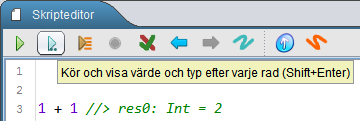
\includegraphics[width=12.0cm]{../img/show-value.png}
\section*{\color{OliveGreen}Tip:}


\begin{itemize}

\item {\lstinline{/} between integers creates a division of integers and the decimals will be ignored. To make a division with decimals, at least one of the numbers must contain decimals.}
\item {With \lstinline{%} you get the rest of a division of integers.}

\end{itemize}


\end{multicols}

\chapter{Name the values with \lstinline{val}}
\begin{multicols}{2}
\section*{\color{BrickRed}Challenge:}
With \lstinline{val} you can connect a name to a value. The name could then be used instead of the value. Try out the program below. What does the turtle write?

\begin{lstlisting}[numbers=none]
val x = 10
val y = 5
val cucumber = x + y
val banana = x * y

clear
forward; write(banana)
forward; write(cucumber)
forward; write(y)
forward; write(x)
\end{lstlisting}
        

\columnbreak

\begin{center}
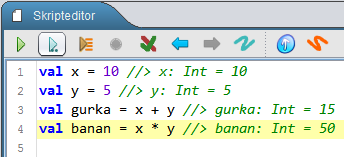
\includegraphics[width=12.0cm]{../img/val.png}
\end{center}

\end{multicols}

\chapter{Random numbers}\section*{\color{BrickRed}Challenge:}


\begin{itemize}

\item {Run the program below several times. What happens?}
\item {What is the smallest and largest possible value of the radius \lstinline{r}?}
\item {Change it so that \lstinline{r} becomes a random number between 3 and 200.}
\item {Draw 100 circles with random radiuses on random positions, as shown in the picture.}

\end{itemize}



\begin{tikzpicture}[overlay]
\node at (21.0cm,-5.0cm) {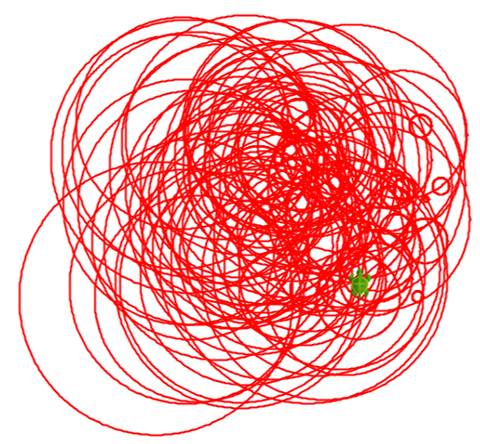
\includegraphics[width=8.0cm]{../img/random-circles.png}};
\end{tikzpicture}
  

\begin{lstlisting}[basicstyle={\ttfamily\fontsize{20}{24}\selectfont},numbers=none]
//r becomes a random number between 10 and 89:
val r = random(90) + 10   

clear; setAnimationDelay(10); invisible
write("Radius = " + r)
circle(r)
\end{lstlisting}
        
\chapter{Mix your own colors}

\begin{itemize}

\item {You can mix your own colors with \lstinline{Color}, for example \lstinline{Color(0, 70, 0)}}
\item {The three parameters are the values for {\it red}, {\it green} och {\it blue}}
\item {You are also able to add a fourth parameter that gives the {\it transparency}}
\item {All parameters are between 0 and 255}

\end{itemize}


\section*{\color{BrickRed}Challenge:}
Try the program below. Change the transparency

\begin{tikzpicture}[overlay]
\node at (23.0cm,-2.0cm) {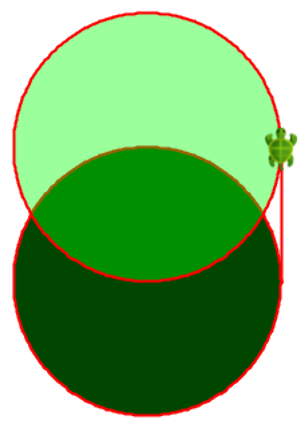
\includegraphics[width=7.0cm]{../img/color-circles.png}};
\end{tikzpicture}
  

\begin{lstlisting}[basicstyle={\ttfamily\fontsize{16}{19}\selectfont},numbers=none]
clear; setAnimationDelay(100)      

val olivegreen = Color(0,70,0)
val pistageicecream = Color(0,255,0,100)

setFillColor(olivegreen); circle(100)
setFillColor(pistageicecream); forward(100); circle(100)
\end{lstlisting}
        
\chapter{Try the color chooser}
\begin{multicols}{2}
\section*{\color{BrickRed}Challenge:}


\begin{itemize}

\item {Rightclick in the editorwindow and click \lstinline{Choose color...}}
\item {If you choose the tab {\bf RGB} in the colourpicker you can pick amongst new RGB-colors.}
\item {Press OK and look in the outputwindow. There you can see the three RGB-values for red, green and blue.}
\item {You can use these values in your program to draw your new color with \lstinline{color(Color(218,153,67))}.}

\end{itemize}



\columnbreak

\begin{center}
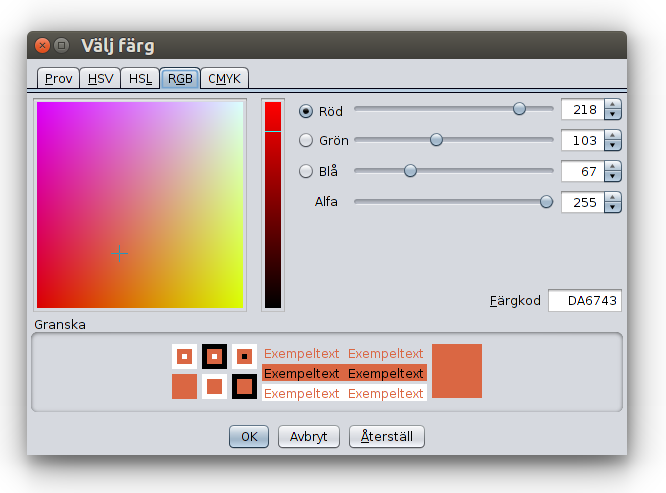
\includegraphics[width=14.0cm]{../img/color-chooser-rgb-sv.png}
\end{center}

\end{multicols}

\chapter{Draw random circles}
\begin{multicols}{2}

\begin{lstlisting}[basicstyle={\ttfamily\fontsize{16}{19}\selectfont},numbers=none]
def random = random(256)
def randomsetPenColor = Color(random,10,random,100) 

clear; setAnimationDelay(5)
setBackground2(black,white)
setPenThickness (6)

repeat(100) {
    setPenColor(randomsetPenColor)
    circle(100)
    hop(20)
    right(35)
}
\end{lstlisting}
        
\section*{\color{BrickRed}Challenge:}
Try different randomcolors and backgrounds.


\columnbreak


\begin{center}
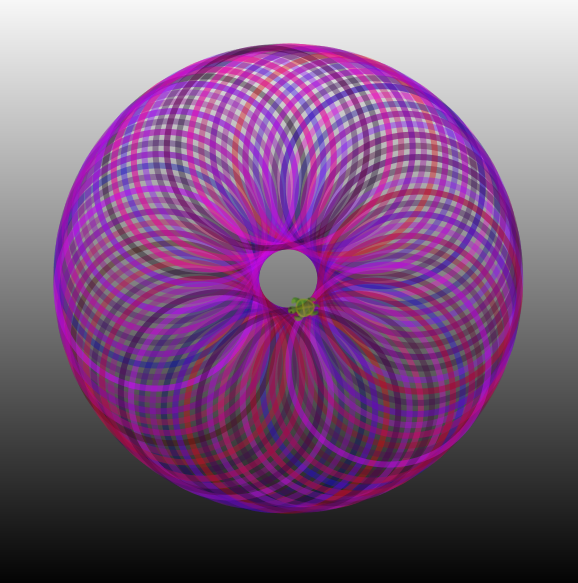
\includegraphics[width=12.0cm]{../img/circle-of-circles.png}
\end{center}

\end{multicols}

\chapter{Draw a flower}\section*{\color{BrickRed}Challenge:}
The program below draws 100 randomcolored circles in a random place with a random radius. Try to change the parameters and try to explain what is happening.

\begin{tikzpicture}[overlay]
\node at (22.0cm,-4.0cm) {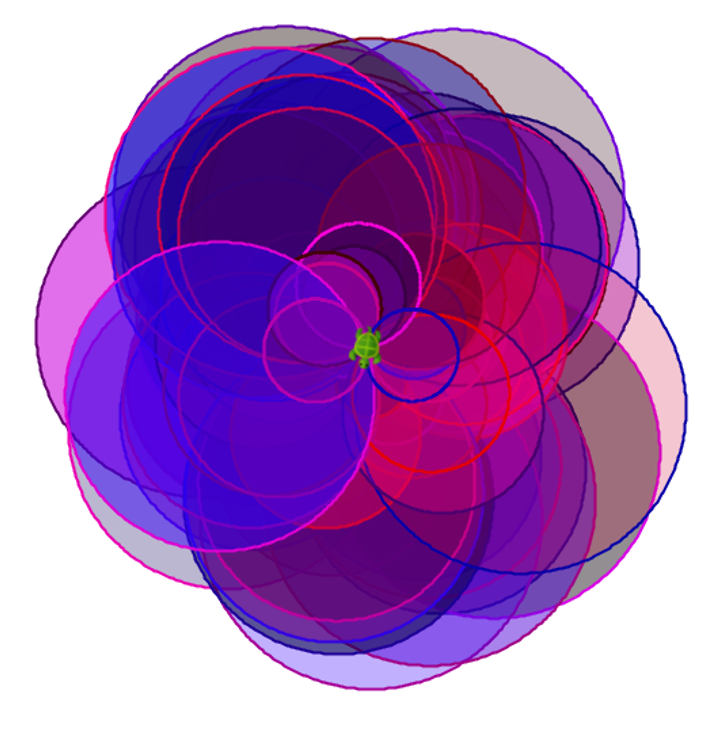
\includegraphics[width=8.5cm]{../img/random-color-circles.png}};
\end{tikzpicture}
  

\begin{lstlisting}[basicstyle={\ttfamily\fontsize{16}{19}\selectfont},numbers=none]
clear(); setAnimationDelay(5)
setPenThickness (2)
repeat(100){
  setPenColor(Color(random(256),0,random(256)))
  setFillColor(Color(random(256),0,random(256),random(100)+50))
  left(random(360))
  circle(random(30)*4+10)
}
\end{lstlisting}
        
\chapter{Create a variable with \lstinline{var}}With \lstinline{var} you connect a name to a value.\\
You get a variable that you can assign a value like this:

\begin{lstlisting}[numbers=none]

var cucumber = 1
cucumber = 1 + 1   //first it calculates 1 + 1 and then assigns that number to cucumber     
        
\end{lstlisting}
        
\section*{\color{BrickRed}Challenge:}
Try the program below. What does the turtle write?

\begin{lstlisting}[basicstyle={\ttfamily\fontsize{16}{19}\selectfont},numbers=none]
var i = 0

clear
repeat(10){
  i = i + 1
  forward; write(i)
}
\end{lstlisting}
        
\section*{\color{OliveGreen}Tip:}


\begin{itemize}

\item {In the command \lstinline{i = i + 1} \lstinline{i} is given the new value which becomes the {\it old} value of \lstinline{i} plus \lstinline{1}}

\end{itemize}


\chapter{Draw many flowers}\section*{\color{BrickRed}Challenge:}


\begin{itemize}

\item {Make a function called \lstinline{flower}, that paints a crown and a stalk from the crowns middle with a green leaf.}
\item {Draw 5 flowers next to each other.}

\end{itemize}



\begin{tikzpicture}[overlay]
\node at (15.0cm,-7.0cm) {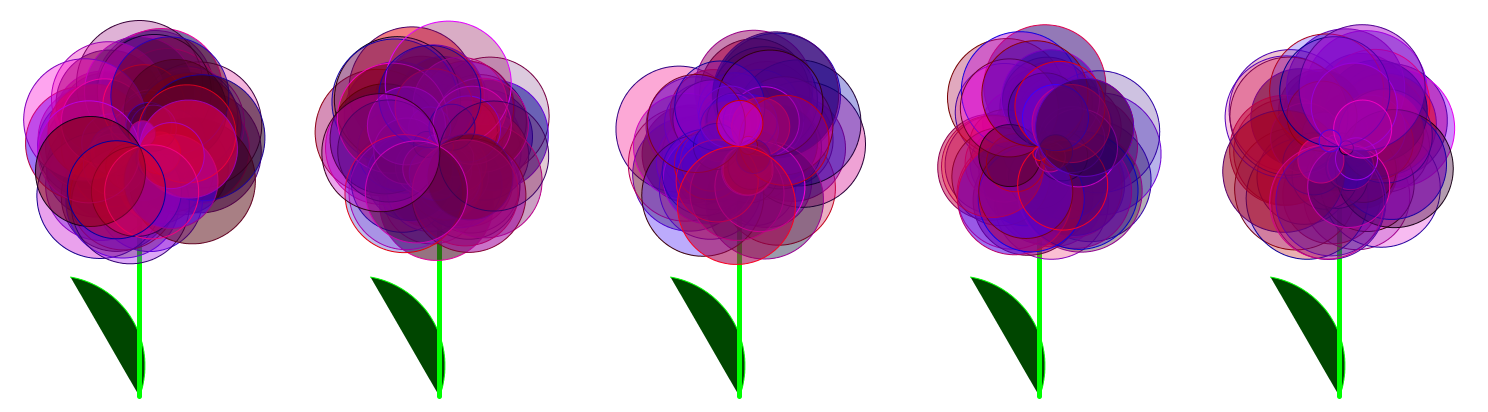
\includegraphics[width=16.0cm]{../img/flowers.png}};
\end{tikzpicture}
  
\section*{\color{OliveGreen}Tip:}
You can draw leafs with \lstinline{bow(radie, vinkel)}. \\
Let the function \lstinline{flower.} have two parameters, x and y, and use \lstinline{jumpTo(x,y)}\\
You can loop 5 times and calculate the position like this:

\begin{lstlisting}[basicstyle={\ttfamily\fontsize{18}{22}\selectfont},numbers=none]
var i = 0          
repeat(5){
  flower(600*i,0)
  i = i + 1        
}
\end{lstlisting}
        
\chapter{Change costume on the turtle}\section*{\color{BrickRed}Challenge:}
Download the mediafiles from Kojos homepage:
\href{http://www.kogics.net/kojo-download#media}{www.kogics.net/kojo-download\#media}


\begin{itemize}

\item {Unzip the file \lstinline{scratch-media.zip} and find the crabpicture \lstinline{crab1-b.png} in the folder \lstinline{Media/Costumes/Animals}}
\item {Put the file \lstinline{crab1-b.png} in the same folder as your program.}
\item {Try changing the costume of the turtle to a crab like this:}

\end{itemize}



\begin{tikzpicture}[overlay]
\node at (12.0cm,-2.5cm) {
\includegraphics[width=4.0cm]{../img/crab1-b.png}};
\end{tikzpicture}
  

\begin{lstlisting}[basicstyle={\ttfamily\fontsize{20}{24}\selectfont},numbers=none]
clear
setCostume ("crab1-b.png")  
setAnimationDelay(2000)
forward(1000)
\end{lstlisting}
        
\section*{\color{OliveGreen}Tip:}


\begin{itemize}

\item {You can also use your own pictures of the types \lstinline{.png} or \lstinline{.jpg}}
\item {If you want to put the picture in another folder you have to write the path to the file, for example \lstinline{kostym("~/Kojo/Media/Costumes/Animals/crab1-b.png")} where \lstinline{~} means your homefolder.}

\end{itemize}


\chapter{Make many turtles with \lstinline{new}}You can create many new turtles with \lstinline{new} like this:

\begin{lstlisting}[basicstyle={\ttfamily\fontsize{18}{22}\selectfont},numbers=none]
clear
val p1 = new Turtle(100,100) //the new turtle p1 starts on position (100, 100)
val p2 = new Padda(100, 50)  //the new turtle p2 starts on position (100, 50)
p1.forward(100)
p2.forward(-100)  //turtle p2 backs up
\end{lstlisting}
        

\begin{tikzpicture}[overlay]
\node at (22.0cm,-2.0cm) {
\includegraphics[width=5.0cm]{../img/new.png}};
\end{tikzpicture}
  
\section*{\color{BrickRed}Challenge:}


\begin{itemize}

\item {Create three turtles that stand above each other.}
\item {Make all their heads turn left.}

\end{itemize}


\section*{\color{OliveGreen}Tip:}


\begin{itemize}

\item {\lstinline{p1} and \lstinline{p2} are the turtles {\it names}. You can pick any name you want.}
\item {With the name \lstinline{p1} and a dot you can give a specific turtles instructions, like this: \lstinline{p1.left}}
\item {\lstinline{invisible} turns the ordinary turtle invisible.}

\end{itemize}


\chapter{Make a race}
\begin{multicols}{2}
With the help of randomnumber you can make the turtles race each other
\section*{\color{BrickRed}Challenge:}


\begin{itemize}

\item {Let three turtles race.}
\item {If they all run forward 10 times, which turtle will win?}

\end{itemize}


\section*{\color{OliveGreen}Tip:}


\begin{itemize}

\item {With \lstinline{p1.forward(randomtal(100) + 1)} the turtle p1 moves 1 to 100 steps forward}

\end{itemize}



\columnbreak

\begin{center}
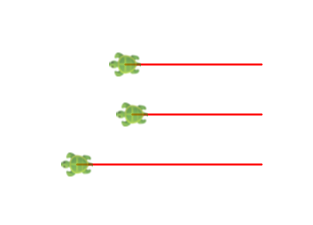
\includegraphics[width=12.0cm]{../img/race.png}
\end{center}

\end{multicols}

\chapter{Alternative with \lstinline{if}}With an \lstinline{if}-command the computer picks between two different alternatives.

\begin{lstlisting}[basicstyle={\ttfamily\fontsize{20}{24}\selectfont},numbers=none]
clear; invisible
if (true) write("true") else write("false")
\end{lstlisting}
        
\section*{\color{BrickRed}Challenge:}


\begin{itemize}

\item {Change \lstinline{true} to \lstinline{false} and check what the turtle writes.}
\item {Change the condition to \lstinline{2 > 1} and check what the turtle writes.}
\item {Change the condition to \lstinline{2 < 1} and check what the turtle writes.}
\item {Explain how an \lstinline{if}-command works.}

\end{itemize}


\section*{\color{OliveGreen}Tip:}


\begin{itemize}

\item {If the condition after  \lstinline{if} is \lstinline{true} whatever is after that condition is picked.}
\item {If the condition after  \lstinline{if} is \lstinline{false} whatever is after \lstinline{else} is picked.}

\end{itemize}


\chapter{React to what the user is doing}
\begin{lstlisting}[basicstyle={\ttfamily\fontsize{20}{24}\selectfont},numbers=none]
clearOutput; setOutputTextFontSize(35)
val password = "cucumber"
val question     = "What is the password?"
val right      = "The safe is open!"
val wrong       = "You may not come in!"
val answer = readln(answer)  //waits for an answer from the user
val message = if (answer == password) right else wrong
println(message)
\end{lstlisting}
        
\section*{\color{BrickRed}Challenge:}


\begin{itemize}

\item {Try the program and explain what happens.}
\item {Change the password, question and what is printed when the question is right and wrong.}
\item {Also ask for a usernamn and add it to what is printed.}

\end{itemize}


\chapter{Make a \lstinline{while}-loop}With a \lstinline{while}-loop the computer will repeat a command as long as the condition is true.

\begin{lstlisting}[basicstyle={\ttfamily\fontsize{22}{27}\selectfont},numbers=none]
clear; invisible; setAnimationDelay(250); clearOutput
var x = 200
while (x > 0) {  //checks the condition before every run 
  forward(x); right
  write(x) 
  x = x - 12
}
println("x is now: " + x)
\end{lstlisting}
        
\section*{\color{BrickRed}Challenge:}


\begin{itemize}

\item {What is printed in the outputwindow? Why?}
\item {Trace the program with the orange-colored play-button and check every step.}
\item {Change the reduction of \lstinline{x} from \lstinline{12} to \lstinline{20}. Explain what happens.}

\end{itemize}


\chapter{Guess the number}
\begin{lstlisting}[basicstyle={\ttfamily\fontsize{16}{19}\selectfont},numbers=none]
val secretNumber = random(100)+1
var answer = readln("Guess a number between 1 and 100! ")
var continue = true

while (continue) {
    if (answer.toInt < secretNumber)
      answer = readln(answer + " is too SMALL, guess again!")
    else if (answer.toInt > secretNumber)
      answer = readln(answer + " is too LARGE, guess again!")
    else if (answer.toInt == secretNumber)
      continue = false
}
println(secretNumber + " is the CORRECT answer!")
\end{lstlisting}
        
\section*{\color{BrickRed}Challenge:}
Introduce a variable \lstinline{var amountOfTries = 0} and make sure to print:\\
\lstinline{Correct answer! You got it in 5 guesses}
\chapter{Practice multiplication}
\begin{lstlisting}[basicstyle={\ttfamily\fontsize{16}{19}\selectfont},numbers=none]
var rightAnswers = 0
val startTime = System.currentTimeMillis / 1000
repeat(12) {
  val number1 = random(12)+1
  val number2 = random(12)+1
  val answer = readln("What is  " + number1 + "*" + number2 + "?")
  if (answer == (number1 * number2).toString) {
    println("Correct!")
    rightAnswers = rightAnswers + 1
  }
  else println("Wrong. The right answer is " + (number1 * number2))
}
val stopTime = System.currentTimeMillis / 1000
val sec = stopTime - startTime
println("You got " + rightAnswers + " right answer in " + sec + " seconds")
\end{lstlisting}
        
\section*{\color{BrickRed}Challenge:}
Change so that you only practice on multiplications of 8 and 9.
\chapter{Save the animals in a vector}
\begin{lstlisting}[basicstyle={\ttfamily\fontsize{14}{17}\selectfont},numbers=none]
var animal = Vector("elk", "cow", "rabbit", "mite")  // the variable animal becomes a vector with 4 animals
println("The first animal in the vector is: " + animal(0))     //the positions in a vector are counted from 0
println("The second animal in the vector is:  " + animal(1))
println("There are these many animals in the vector: " + animal.size)
println("The last animal in the vector is:  " + animal(animal.size-1))

val s = random(animal.size)   //take a random number between 0 and the number of animals minus 1
println("A random animal: " + animal(s))
animal = animal :+ "camel"    //adds another animal last in the vector
animal = "dromedary" +: animal // adds another animal first in the vector

animal = animal.updated(2, "mudskipper")  // Change the third animal(index 2 in vector)
println("All animals in the array backwards:")
animal.foreach{ x => println(x.reverse) } // for all x in array: type out x backwards.
\end{lstlisting}
        
\section*{\color{BrickRed}Challenge:}


\begin{itemize}

\item {What does the program print out in the output window? Explain what's happening.}
\item {Add more animals to the array.}

\end{itemize}


\chapter{Practice words}
\begin{lstlisting}[basicstyle={\ttfamily\fontsize{14}{17}\selectfont},numbers=none]
val Swedish = Vector("dator", "sköldpadda", "cirkel")
val English = Vector("computer", "turtle", "circle")
var amountRight = 0
repeat(5) {
  val s = random(3)
  val word = Swedish(s)
  val answer = readln("What is " + word + " in English?")
  if (answer == English(s)) {
    println("Correct answer!")
    amountRight = amountRight + 1
  } else {
    println("Wrong answer. Correct answer is: " + English(s))
  }
}
println("You have" + amountRight + " correct answers.")
\end{lstlisting}
        
\section*{\color{BrickRed}Challenge:}


\begin{itemize}

\item {Add more words.}
\item {Practice words from English to Swedish.}
\item {Let the user choose how many questions before end. Tip: \lstinline{val amount = input("Amount: ").toInt} }

\end{itemize}


\chapter{Capital Game}
\begin{lstlisting}[basicstyle={\ttfamily\fontsize{13}{16}\selectfont},numbers=none]
def capitalGame = {
  println("Welcome to the Capital Game!")
  val city = Map("Sweden" ->"Stockholm", "Denmark" -> "Copenhagen", "Skåne" -> "Malmö")
  var countriesLeft = city.keySet //keySet gives an amount of all keys in a Map 
  def randomCountry = scala.util.Random.shuffle(countriesLeft.toVector).head
  while(!countriesLeft.isEmpty) {
    val country = randomCountry
    val answer = input("What is the capital in " + country + "?")
    output(s"You wrote: $answer")
    if (answer == city(country)) {
      output("Correct answer! You have " + countriesLeft.size + " countries left!")
      countriesLeft = countriesLeft - country  //remove country from the set of countries left
    } else output(s"Wrong answer. The capital in $country begins with ${city(country).take(2)}...")
  }
  output("THANK YOU FOR PLAYING! (Press ESC)")
}

toggleFullScreenOutput;  
setOutputBackground(black); setOutputTextColor(green); setOutputTextFontSize(30)
repeat(100)(output("")) //scroll the output window with 100 blank rows.
capitalGame

// *** TASK: (1) Add more pairs of countries and cities: country -> city (2) Measure time and count points.
\end{lstlisting}
        
\chapter{Make a timer with \lstinline{object}}
\begin{lstlisting}[basicstyle={\ttfamily\fontsize{14}{17}\selectfont},numbers=none]
object timer {
  def now = System.currentTimeMillis  //gives time now in milliseconds.
  var time = now
  def reset = { time = now }
  def measure = now - time
  def randomWait(min: Int, max: Int) =  //wait between min and max seconds
    Thread.sleep((random(max-min)+min)*1000)  //Thread.sleep(1000) waits 1 second
}

println("Click in the println window and wait...")
timer.randomWait(3,6)   //wait between 3 and 6 seconds
timer.reset
readln("Press Enter as fast as you can.")
println("Reaction time: " + (timer.measure/1000.0) + " seconds")
\end{lstlisting}
        
With \lstinline{object}  you can collect things that belong together into an object.\\
 You can reach a thing inside an object with a dot: \lstinline{timer.reset}
\section*{\color{BrickRed}Challenge:}


\begin{itemize}

\item {Try the program and measure your reaction time. How fast are you?}
\item {Use \lstinline{timer} in the task {\it Guess the number} and add the print-out: \lstinline{Correct answer! You made it in 5 guesses and 32 seconds}}

\end{itemize}


\chapter{Simulate a traffic light}
\begin{tikzpicture}[overlay]
\node at (22.0cm,-6.0cm) {
\includegraphics[width=3.0cm]{../img/traffic-lights.png}};
\end{tikzpicture}
  

\begin{lstlisting}[basicstyle={\ttfamily\fontsize{14}{17}\selectfont},numbers=none]
def turnOffAll = draw(penColor(gray) * fillColor(black) -> PicShape.rect(130,40))
def light(c: Color, h: Int) = penColor(noColor) * fillColor(c) * trans(20,h) -> PicShape.circle(15)
def lightRed = draw(light(red, 100))
def lightYellow = draw(light(yellow, 65))
def lightGreen = draw(light(green, 30))
def wait(seconds: Int) = Thread.sleep(seconds*1000)

clear; invisible  
while (true) { //an infinite loop
  turnOffAll
  lightRed;  wait(3)
  lightYellow;  wait(1) 
  turnOffAll
  lightGreen; wait(3)
  lightYellow;  wait(1)
}
\end{lstlisting}
        
\section*{\color{BrickRed}Challenge:}


\begin{itemize}

\item {How does the traffic light switch? Try explaning what's happening.}
\item {Change so that the green light is on for the double amount of time.}

\end{itemize}


\chapter{Control the turtle with the keyboard}
\begin{multicols}{2}

\begin{lstlisting}[basicstyle={\ttfamily\fontsize{18}{22}\selectfont},numbers=none]
clear; setAnimationDelay(0)
activateCanvas()

animate { forward(1) }

onKeyPress { k =>
  k match {
    case Kc.VK_LEFT =>   left(5)
    case Kc.VK_RIGHT =>  right(5)
    case Kc.VK_SPACE =>  forward(5)
    case _ => 
      println("Another key: " + k)
  }
}
\end{lstlisting}
        


\columnbreak


\section*{\color{BrickRed}Challenge:}


\begin{itemize}

\item {Write \lstinline{Kc.} and press \lstinline{Ctrl+Alt+Space} and look up what the different keys are called.}
\item {Do \lstinline{penUp} if you press the arrow up key}
\item {Do \lstinline{penUp} if you press the arrow down key}
\item {Do \lstinline{color(blue)} if you press B}
\item {Do \lstinline{color(red)} if you press R}
\item {Increase or decrease the speed if you press + or -}

\end{itemize}


\end{multicols}

\chapter{Control the turtle with the mouse}
\begin{multicols}{2}

\begin{lstlisting}[basicstyle={\ttfamily\fontsize{16}{19}\selectfont},numbers=none]
clear; setAnimationDelay(100)
activateCanvas()

var draw = true

onKeyPress { k =>
  k match {
    case Kc.VK_DOWN => 
      penDown()
      draw = true
    case Kc.VK_UP => 
      penUp()
      draw = false
    case _ => 
      println("Another key: " + k)
  }
}

onMouseClick { (x, y) =>
  if (draw) moveTo(x, y) else jumpTo(x, y)
}
\end{lstlisting}
        


\columnbreak


\section*{\color{BrickRed}Challenge:}


\begin{itemize}

\item {Do \lstinline{setFillColor(black)} if you press the key F}
\item {Introduce a variable \lstinline{var fillNext = true} and in the case you press \lstinline{Kc.VK_F} do:}

\end{itemize}



\begin{lstlisting}[numbers=none]

      if (fillNext) {
        setFillColor(black)
        fillNext=false
      } else {
        setFillColor(noColor)
        fillNext=true
      }
      
\end{lstlisting}
        
\end{multicols}

\chapter{Make your own bank account}
\begin{multicols}{2}

\begin{lstlisting}[basicstyle={\ttfamily\fontsize{16}{19}\selectfont},numbers=none]
object myAccount {
  val number = 123456
  var balance = 0.0
  def in(amount: Double) = {
    balance = balance + amount 
  }
  def out(amount: Double) = { 
    balance = balance - amount 
  }
  def showBalance() = {
    println("Account number: " + number) 
    println("       Balance: " + balance)
  }
}

myAccount.showBalance()
myAccount.in(100)
myAccount.showBalance()
myAccount.out(10)
myAccount.showBalance()
\end{lstlisting}
        


\columnbreak


\section*{\color{BrickRed}Challenge:}


\begin{itemize}

\item {What is the balance after the program has finished? Explain what's happening.}
\item {Make it impossible to withdraw more than there is in the account.}
\item {Add \lstinline{val maxAmount = 5000} and make sure you can't withdraw more than \lstinline{maxBelopp} at a time.}

\end{itemize}


\end{multicols}

\chapter{Make many objects from a \lstinline{class}}
\begin{multicols}{2}
A class is needed to make many accounts. With \lstinline{new} new objects are made. Each object gets a number and balance.

\begin{lstlisting}[basicstyle={\ttfamily\fontsize{13}{16}\selectfont},numbers=none]
class Account(number: Int) {
  private var balance = 0.0 //private means "secret"  
  def in(amount: Double) = {
    balance = balance + amount
  }
  def out(amount: Double) = {
    balance = balance - amount
  }
  def showBalance() = 
    output(s"Account $number: $balance")
}

val account1 = new Account(12345) //new makes an object
val account2 = new Account(67890) //another object

account1.in(99)
account2.in(88)
account1.out(57)
account1.showBalance
account2.showBalance
\end{lstlisting}
        


\columnbreak


\section*{\color{BrickRed}Challenge:}


\begin{itemize}

\item {What is the balance on the different accounts when the program has finished? Explain what's happening.}
\item {Make even more Account objects and deposit and withdraw money from these.}
\item {Add a class parameter \lstinline{name: String} containing the name of the owner of the bankaccount.}
\item {Do that even the \lstinline{name} is printed when \lstinline{showBalance} is called}
\item {What happens if you do: \lstinline{account1.balance = 10000000 }}

\end{itemize}


\end{multicols}

\chapter{Talk to the computer}
\begin{lstlisting}[basicstyle={\ttfamily\fontsize{13}{16}\selectfont},numbers=none]
setOutputBackground(black); setOutputTextFontSize(30); setOutputTextColor(green)
println("Write interesting answers even if the questions are weird. End with 'good bye'")
def randomize(xs: Vector[String]) = scala.util.Random.shuffle(xs).head
val text = Vector("What does this mean: ", "Do you like", "Why is this needed: ", "Tell more about")
var answer = "?"
val opening = "What do you want to talk about?"
var word = Vector("bellybutton fluff", "ketchup-icecream", "Santa Claus", "pillow") 
while (answer != "good bye") {
  val t = if (answer == "?") opening 
    else if (answer == "No") "Well, no." 
    else if(answer == "Yes") "Well, yes." 
    else if (answer.length < 4) "Okay..." 
    else randomize(text) + " " + randomize(word) + "?"
  answer = readln(t).toLowerCase
  word = word ++ answer.split(" ").toList.filter(_.length > 3) 
} 
println("Thanks for the talk! Now I know these words:" + word)

//Task:
// (1) Try the program and explain what's happening.
// (2) When does the while-loop finish?
// (3) Add more strings in the vectors "text" and "word".
// (4) Add more good answers to short words apart from "No" and "Yes".
\end{lstlisting}
        
\chapter{Modify the pong game}
\begin{multicols}{2}
\section*{\color{BrickRed}Challenge:}


\begin{itemize}

\item {Choose the menu Samples > Animations and Games > Pong and try the game.}
\item {You control with the up and down arrows,  A and Z.}
\item {Press ESC to cancel the game and examine the code.}
\item {Change the code so that the ball becomes bigger.}
\item {Make the playing field to a tennis field, with green background, white lines and a yellow ball.}

\end{itemize}



\columnbreak

\begin{center}
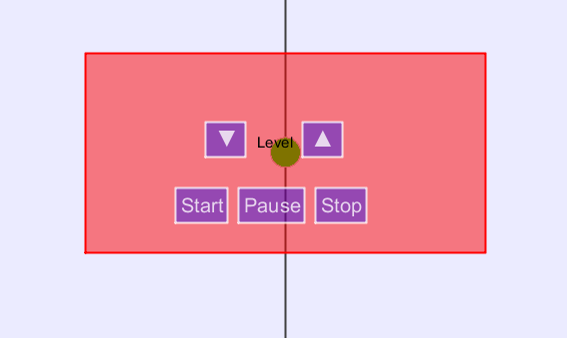
\includegraphics{../img/pong.png}
\end{center}

\end{multicols}

  %%%LOCALIZE

\end{document}